\documentclass[pdftex,12pt,xcolor=svgnames]{beamer}

\mode<presentation>
{
  \usetheme{boxes}
  \usecolortheme[named=MidnightBlue]{structure}
  %\setbeamercolor{normal text}{bg=NavajoWhite!20}
  \usefonttheme{serif}
  \setbeamertemplate{navigation symbols}{}
  % Show frame number and author name in footline
  \setbeamertemplate{footline}[frame number]
  \addtobeamertemplate{footline}{\quad\textcolor{gray}{James Robert Lloyd}}{}
  % Set frame titles in small capitals
  \setbeamerfont{frametitle}{shape=\scshape,family=\rmfamily}
  \setbeamercolor{frametitle}{bg=gray!60!white,fg=black}
  % Alerted text: blue (uncomment second line if theme sets alerted text to bold)
  \setbeamercolor{alerted text}{fg=blue}
  %\setbeamerfont*{alerted text}{}
  \setbeamertemplate{bibliography item}[text] %{\hbox{\donotcoloroutermaths$\blacktriangleright$}}
  \setbeamertemplate{bibliography entry title}{}
  \setbeamertemplate{bibliography entry author}{}
  \setbeamertemplate{bibliography entry note}{}
  \setbeamertemplate{bibliography entry location}{}

}
\usepackage[english]{babel}
\usepackage[latin1]{inputenc}
\usepackage{times}
\usepackage[T1]{fontenc}
\usepackage{hyperref}
\usepackage{multimedia}
\usepackage{eepic}
\usepackage{graphicx}
%\usepackage[nohug]{latexinclude/diagrams}
\usepackage{tikz}
\usetikzlibrary{calc}

%% \newcommand{\footlineextra}[1]{
%%     \begin{tikzpicture}[remember picture,overlay]
%%         \node[yshift=1.5ex,anchor=south east] at (current page.south east)
%% {#1};
%%     \end{tikzpicture}
%% }

\newcommand{\footlineextra}[1]{
    \begin{tikzpicture}[remember picture,overlay]
        \node[xshift=-5ex,yshift=-0.5ex,anchor=south east] at (current page.south east)
             {\mbox{\tiny \textcolor{MidnightBlue}{#1}}};
    \end{tikzpicture}
}

\def\sectionframe#1{
  {
    \setbeamertemplate{footline}{\empty}
    \begin{frame}{}
      \begin{center}
        \huge\sc #1
      \end{center}
    \end{frame}
  }
}


\usepackage{etex}

\usepackage{tabularx}
\usepackage{include/picins}
\usepackage{include/preamble}
\usepackage{tikz}

\usetikzlibrary{shapes.geometric,arrows,chains,matrix,positioning,scopes,calc}

%%%%%%%%%%%%%%%%%%%%%%%%%%%%%%%%%%%%%%%%%%%
%
% Some look and feel definitions
%
%%%%%%%%%%%%%%%%%%%%%%%%%%%%%%%%%%%%%%%%%%%

\setlength{\columnsep}{0.03\textwidth}
\setlength{\columnseprule}{0.0018\textwidth}
\setlength{\parindent}{0.0cm}

\tikzstyle{mybox} = [draw=white, rectangle]

\definecolor{camlightblue}{rgb}{0.601 , 0.8, 1}
\definecolor{camdarkblue}{rgb}{0, 0.203, 0.402}
\definecolor{camred}{rgb}{1, 0.203, 0}
\definecolor{camyellow}{rgb}{1, 0.8, 0}
\definecolor{lightblue}{rgb}{0, 0, 0.80}
\definecolor{white}{rgb}{1, 1, 1}
\definecolor{whiteblue}{rgb}{0.80, 0.80, 1}

\newcolumntype{x}[1]{>{\centering\arraybackslash\hspace{0pt}}m{#1}}
\newcommand{\tabbox}[1]{#1}

\hypersetup{colorlinks=true,citecolor=blue}

%%%%%%%%%%%%%%%%%%%%%%%%%%%%%%%%%%%%%%%%%%%
%
% The talk
%
%%%%%%%%%%%%%%%%%%%%%%%%%%%%%%%%%%%%%%%%%%%

\title{Building an automatic statistician}

\author{
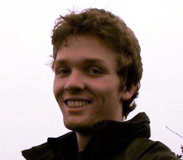
\includegraphics[height=0.2\textwidth]{figures/JamesLloyd4}
\qquad
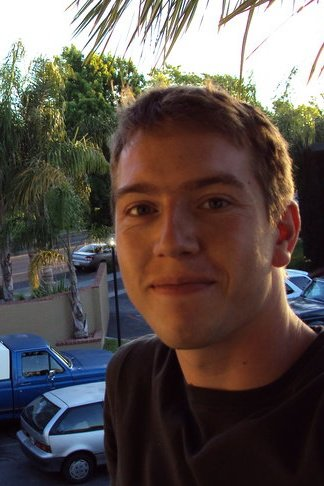
\includegraphics[height=0.2\textwidth, trim=20mm 25mm 0mm 25mm, clip]{figures/david2}
\qquad
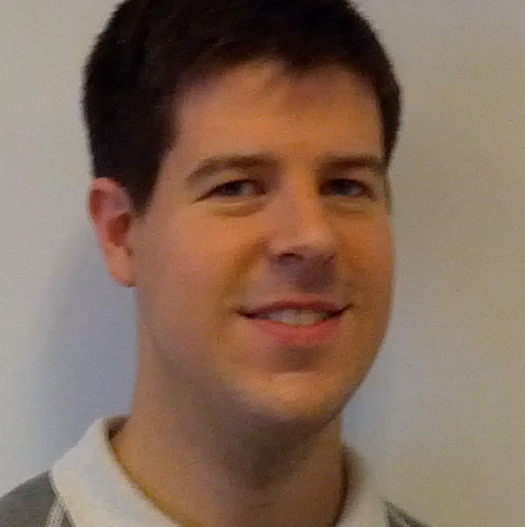
\includegraphics[height=0.2\textwidth]{figures/roger-photo}
\\
James Robert Lloyd, David Duvenaud, Roger Grosse,\\
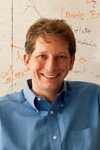
\includegraphics[height=0.2\textwidth, trim=0mm 7mm 0mm 0mm, clip]{figures/josh2}
\qquad
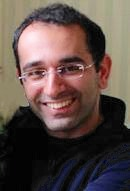
\includegraphics[height=0.2\textwidth]{figures/zg2}\\
Joshua Tenenbaum, Zoubin Ghahramani
}

\begin{document}

\frame[plain] {
\titlepage
}

\begin{frame}{There is a growing need for data scientists}
  \begin{itemize}
    \item We live in an era of abundant data
    \vspace{\baselineskip}
    \item The McKinsey Global Institute claim
    \begin{itemize}
      \item \emph{``The United States alone faces a shortage of 140,000 to 190,000 people with analytical expertise and 1.5 million managers and analysts with the skills to understand and make decisions based on the analysis of big data.''}
    \end{itemize}
    \vspace{\baselineskip}
    \item Automating statistical modeling would mitigate this requirement and potentially have a large impact on fields relying on expert statisticians, machine learning researchers and data scientist
    \begin{itemize}
       \item \eg Computational biology
       \item \emph{Another canonical example} \ldots
     \end{itemize}
  \end{itemize}
\end{frame}

\begin{frame}{Ingredients of an automatic statistician}
  \begin{itemize}
    \item {\bf An open-ended language of models}
    \begin{itemize}
       \item Expressive enough to capture real-world phenomena\ldots
       \item \ldots and the techniques used by human statisticians
     \end{itemize}
    \vspace{\baselineskip}
    \item {\bf A search procedure}
    \begin{itemize}
       \item To efficiently explore the language of models
     \end{itemize}
    \vspace{\baselineskip}
    \item {\bf A principled method of evaluating models}
    \begin{itemize}
       \item Trading off complexity and fit to data
     \end{itemize}
    \vspace{\baselineskip}
    \item {\bf A procedure to automatically explain the models}
    \begin{itemize}
       \item Making the assumptions of the models explicit\ldots
       \item \ldots in a way that is intelligible to non-experts
     \end{itemize}
  \end{itemize}
\end{frame}

\begin{frame}{Defining a language of regression models}
  \begin{itemize}
    \item Regression consists of learning a function $f: \mathcal{X} \to \mathcal{Y}$ from inputs to outputs from example input / output pairs
    \vspace{\baselineskip}
    \item Language should include simple parametric forms\ldots
    \begin{itemize}
       \item \eg Linear functions, Polynomials, Exponential functions
     \end{itemize}
    \vspace{\baselineskip}
    \item \ldots as well as functions specified by high level properties
    \begin{itemize}
       \item \eg Smoothness, Periodicity
     \end{itemize}
    \vspace{\baselineskip}
    \item Inference should be tractable for all models in language
  \end{itemize}
\end{frame}

\begin{frame}{Bayesian modeling}
  Placeholder for TMS
  
  Intro to Bayes rule and use in statistics
\end{frame}

\begin{frame}{Bayesian linear regression}
  Placeholder for TMS
  
  Show example of Bayesian linear regression through origin
  
  Prior, Bayes rule, Posterior, Picture one data point at a time
\end{frame}

\begin{frame}{Bayesian linear regression}
  Placeholder for TMS
  
  Show how to rewrite this as a Gaussian distribution
  
  Talk about finite number of sampling points, and that this has a limit
\end{frame}

\begin{frame}{Gaussian process regression}
  Placeholder for TMS
  
  Change the covariance, shows samples of SE, and then show posterior
\end{frame}

\frame[plain]{
\frametitle{Conditional Posterior}
Placeholder for TMS

With SE kernel:
    \begin{figure}
        \includegraphics<1>[width=6cm]{figures/gp_demo/1d_posterior_and_0_data}
        \includegraphics<2>[width=6cm]{figures/gp_demo/1d_posterior_and_1_data}
        \includegraphics<3>[width=6cm]{figures/gp_demo/1d_posterior_and_2_data}
        \includegraphics<4>[width=6cm]{figures/gp_demo/1d_posterior_and_3_data}
        \includegraphics<5>[width=6cm]{figures/gp_demo/1d_posterior_and_4_data}
    \end{figure}
}

\begin{frame}{Gaussian process regression}
  Placeholder for TMS
  
  Therefore let's see how far we can go with kernel functions
\end{frame}

\begin{frame}{We can do this with Gaussian processes}
  \begin{itemize}
    \item \gp{}s are distributions over functions such that any
finite subset of function evaluations, $(f(x_1), f(x_2), \ldots
f(x_N))$, have a joint Gaussian distribution
    \vspace{\baselineskip}
    \item A \gp{} is completely specified by
    \begin{itemize}
      \item Mean function, $\mu(x)=\mathbb{E}(f(x))$
      \item Covariance / kernel function, $\kernel(x,x') = \Cov(f(x),f(x'))$
    \end{itemize}
  \end{itemize}
  Draw a picture?
\end{frame}

\begin{frame}{A language of Gaussian process kernels}
  \begin{itemize}
    \item Marginalizing over an unknown mean function can be equivalently
expressed as a zero-mean \gp{} with a new kernel
  \begin{itemize}
    \item Suppose, ${f(x) \,|\, a \,\sim\, \gp{}(a \times \mu(x), \kernel(x,x'))}$ and $a \,\sim\, \mathcal{N}(0,1)$
    \item Then equivalently, $f(x) \,\sim\, \gp{}(0, \mu(x)\mu(x') + \kernel(x,x'))$
  \end{itemize}
  \vspace{\baselineskip}
  \item We therefore define a language of \gp{} regression models by
specifying a {\bf language of kernels}
  \end{itemize}
\end{frame}

\begin{frame}{The atoms of our language}
  Show pictures of different function types from base kernels
\end{frame}

\begin{frame}{The composition rules of our language}
  Addition and multiplication with pictures
\end{frame}

\begin{frame}{Modeling changepoints}
  Addition and multiplication with pictures
\end{frame}

\begin{frame}{An expressive language of models}
  Table
\end{frame}

\begin{frame}{Exploring the language}
  \begin{itemize}
    \item Large and open ended
    \vspace{\baselineskip}
    \item Need to be efficient
    \vspace{\baselineskip}
    \item Try to mimick human behaviour
  \end{itemize}
\end{frame}

\begin{frame}{A greedy search}
  Make a new example of kernel learning
\end{frame}

\begin{frame}{Model evaluation}
  Need to trade off complexity and model fit
  
  Bayesian Occam's razor
  
  Multiple slides on this
\end{frame}

\begin{frame}{How can we describe a model}
  Motivating example of $\kSE \times \kPer \times \kLin$.
\end{frame}

\begin{frame}{How can we describe a model}
  Show a big expression
\end{frame}

\begin{frame}{How can we describe a model}
  Convert changepoint operator
\end{frame}

\begin{frame}{How can we describe a model}
  Distributes sums over products
\end{frame}

\begin{frame}{How can we describe a model}
  Sums of kernels are sums of products - maths and picture
\end{frame}

\begin{frame}{How can we describe a model}
  Show the build up of an $\kSE \times \kPer \times \kLin \times \boldsymbol\sigma$ kernel starting with the noun and adding modifiers
  
  Then show the underset kernel description
\end{frame}

\begin{frame}{Example: Airline}
\end{frame}

\begin{frame}{Example: Solar}
\end{frame}

\begin{frame}{Example: Call centre}
\end{frame}

\begin{frame}{Example: Sulphuric}
\end{frame}

\begin{frame}{Good predictive performance as well}
  Interpretability / accuracy trade-off rears its annoying head - but both are pretty good :)
\end{frame}

\begin{frame}{Challenges}
  
\end{frame}

\begin{frame}{Current and future directions}
  
\end{frame}

\begin{frame}{Summary}
  
\end{frame}

\end{document}

\begin{frame}{Title}
  \begin{itemize}
    \item Content
    \vspace{\baselineskip}
    \item Content
    \vspace{\baselineskip}
    \item Content
    \begin{itemize}
       \item Content
       \item Content
     \end{itemize}
  \end{itemize}
\end{frame}